\documentclass[conference]{IEEEtran}

% Local builds use tectonic (XeTeX), where IEEEtran's Times font is only found in
% T1 encoding. Harmless under pdfLaTeX/Overleaf.
\usepackage[T1]{fontenc}
\usepackage{cite}
\usepackage{amsmath,amssymb,amsfonts}
\usepackage{graphicx}
\usepackage{textcomp}
\usepackage{xcolor}
\usepackage{tikz}
\usetikzlibrary{positioning,arrows.meta}

% Keep figures and tables close to their surrounding text in the two-column layout.
\setlength{\textfloatsep}{7pt plus 2pt minus 2pt}
\setlength{\floatsep}{6pt plus 2pt minus 2pt}
\setlength{\intextsep}{6pt plus 2pt minus 2pt}
\usepackage{caption}

\begin{document}

\title{Self-Calibrating Vehicle Speed Estimation from Overhead UAV Video}

\author{\IEEEauthorblockN{Sudhanshu Tyagi\IEEEauthorrefmark{1},
Anmol Mangat\IEEEauthorrefmark{2},
Ishita Vaid\IEEEauthorrefmark{1},
Khushi Garg\IEEEauthorrefmark{1} and
Ishaan Singh\IEEEauthorrefmark{2}}
\IEEEauthorblockA{\IEEEauthorrefmark{1}Department of Electronics and Communication Engineering\\
Thapar Institute of Engineering and Technology, Patiala, Punjab, India\\
Email: s.tyagi@thapar.edu, ivaid\_be23@thapar.edu, kgarg3\_be23@thapar.edu}
\IEEEauthorblockA{\IEEEauthorrefmark{2}Department of Computer Science and Engineering\\
Thapar Institute of Engineering and Technology, Patiala, Punjab, India\\
Email: amangat\_be23@thapar.edu, isingh\_be23@thapar.edu}}

\maketitle

\begin{abstract}
Camera-based vehicle speed estimation is a low-cost alternative to radar and lidar, but converting pixel motion into metric speed requires a scale that usually comes from surveyed road distances, manually set pixel-per-metre values, or calibration vehicles of known speed. This paper presents a speed estimation method for overhead (nadir) unmanned aerial vehicle (UAV) video that obtains this scale from the traffic itself. We show that, for a downward-facing camera, metric ground positions depend only on the ratio of camera height to focal length, so neither needs to be known individually.

The ratio is recovered from the apparent widths of tracked cars, using only bounding-box edges perpendicular to the direction of travel and a lower-percentile estimator that counters the one-sided bias of axis-aligned boxes. Vehicles are detected with an aerial-trained YOLO model and tracked with ByteTrack, hover drift is removed by a background-only homography, and speed is obtained from a least-squares fit over a short trajectory window. Each reading is labelled moving, stopped, or unreliable using a geometric noise model, so stationary vehicles and measurement failures remain distinguishable. Vehicles that exceed a speed limit continuously are logged once, with their peak speed and an evidence image, to a cloud database. The method needs no flight metadata, camera intrinsics, or ground measurements.
\end{abstract}

\begin{IEEEkeywords}
Vehicle Speed Estimation, Unmanned Aerial Vehicles, Camera Calibration, Multi-Object Tracking, Intelligent Transportation Systems
\end{IEEEkeywords}

\section{Introduction}

Vehicle speed monitoring is central to road safety and traffic management. Dedicated sensors such as radar and lidar are accurate but costly to acquire and maintain, while cameras are already widely deployed for traffic surveillance \cite{ref1}. Estimating speed from video is therefore an attractive low-cost alternative.

The difficulty lies in converting pixel motion into metric distance. For roadside cameras, perspective makes the metres-per-pixel scale vary across the image, so the camera must be calibrated and a metric scale must be supplied, either from surveyed road distances, manually set pixel-per-metre values, or vehicles of known speed \cite{ref2,ref3,ref4}. These inputs require a site visit or manual set-up for every camera.

Unmanned aerial vehicles (UAVs) offer a different viewpoint. A camera looking straight down removes perspective distortion, sees vehicles without mutual occlusion, and can be deployed quickly over any road section. The metric scale, however, still depends on the camera height and focal length, and in practice neither is reliably known: altitude is usually reported relative to the take-off point rather than the road, and the effective focal length changes with zoom, cropping, and re-encoding. A fixed metres-per-pixel constant is valid for only one altitude and one resolution.

This paper presents a speed estimation method for overhead UAV video that obtains its scale from the traffic itself (Fig.~\ref{fig:demo}). It uses the fact that, for a downward-facing camera, ground positions depend only on the ratio of camera height to focal length. This ratio is estimated from the apparent widths of the cars being tracked, so no flight metadata, camera parameters, or ground measurements are needed.

\begin{figure}[htbp]
\centering
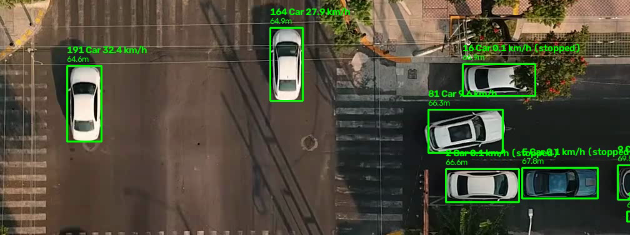
\includegraphics[width=0.98\linewidth]{figs/fig1_drone.png}
\caption{Speed estimates on overhead UAV footage. Moving vehicles carry a measured speed, while parked vehicles are reported as stopped.}
\label{fig:demo}
\end{figure}

\textbf{Key contributions of this work include:} a nadir camera model showing that metric speed depends only on the height-to-focal-length ratio, together with a self-calibration procedure that recovers this ratio from tracked car widths and is robust to the one-sided bias of axis-aligned bounding boxes; an uncertainty-aware speed estimator that labels every reading as moving, stopped, or unreliable, so that stationary vehicles and measurement failures are never confused; and a complete system that compensates for UAV hover drift and logs each speeding vehicle once, with its peak speed and an evidence image, to a cloud database.

% TODO: once Results are added, change to "... Section III presents the
% methodology, Section IV reports the results and analysis, and Section V concludes."
The rest of the paper is organised as follows. Section II reviews related work, Section III presents the methodology, and Section IV concludes.

\section{Related Work}

A common approach to camera-based speed estimation measures how a vehicle moves between virtual lines drawn on the road. Sangsuwan and Ekpanyapong \cite{ref4} defined four intrusion lines and combined YOLOv3, DeepSORT, and optical flow to measure crossing displacement and travel time; the parameters of their speed models were fitted using vehicles whose speeds were measured with a laser speed gun. Mouafo and Biaou \cite{ref1} proposed an uncalibrated approach using YOLOv8 and ByteTrack that estimates the average speed over a known distance between intrusion lines. Both methods avoid full camera calibration but depend on distances or reference speeds measured at the site.

Other methods map image coordinates onto the road plane. Lashkov et al. \cite{ref5} used a projective transformation to compute real-world distances from a fixed intersection camera. Kamil et al. \cite{ref3} rectified monocular video into a bird's-eye view with a deep image homography network and estimated speed over consecutive frames, but the pixel-per-metre value of the rectified view was applied manually. Dubsk\'a et al. \cite{ref2} calibrated roadside cameras fully automatically from vanishing points found in vehicle trajectories, recovering the ground plane and focal length; the scene scale, however, must still be obtained separately.

Camera motion is a further source of error, because any image shift is read as vehicle motion. Lashkov et al. \cite{ref5} addressed wind-induced vibration of surveillance cameras with image-matching algorithms. A hovering UAV faces the same problem in a stronger form, since its position drifts continuously.

Detection and tracking form the front end of these pipelines. YOLO detectors combined with ByteTrack association are widely used \cite{ref1,ref3,ref6}, and Wang and Mariano \cite{ref6} improved YOLOv8s for small targets, which are typical of aerial imagery. Most trackers use a Kalman filter as their motion model, and its efficiency and robustness under occlusion remain active topics \cite{ref7}.

The methods above target fixed roadside cameras and need an external source of metric scale: surveyed line distances, a manually set pixel-per-metre value, or calibration vehicles of known speed. This paper addresses that gap for overhead UAV video by deriving the scale from the observed vehicles themselves.

\section{Methodology}

This section describes the complete pipeline, shown in Fig.~\ref{fig:pipeline}. Vehicles are detected and tracked in every frame, and a one-time calibration estimates the metric scale from the tracked cars. During operation, vehicle positions are corrected for UAV drift, projected onto the road plane, and converted into speeds by a trajectory fit. Each reading then passes a reliability gate, and vehicles that exceed the speed limit are logged.

\begin{figure}[htbp]
\centering
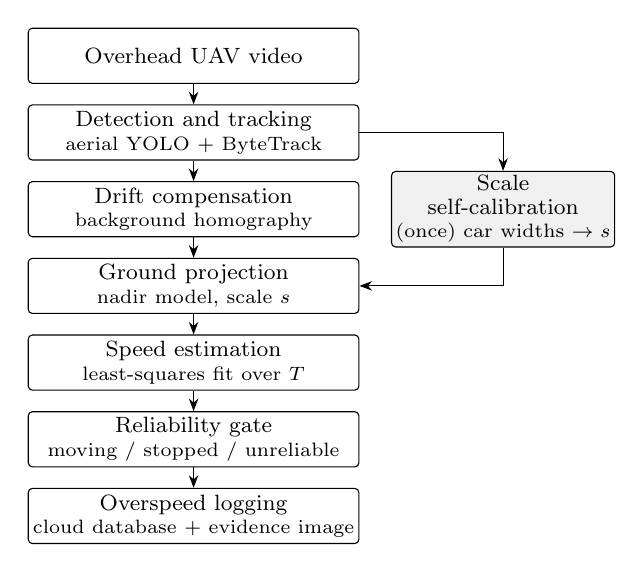
\begin{tikzpicture}[
  node distance=2.6mm,
  >={Stealth[length=1.6mm]},
  box/.style={draw, rounded corners=1.5pt, align=center, font=\footnotesize,
              minimum width=42mm, minimum height=7mm, inner sep=1.5pt},
  side/.style={box, minimum width=25mm, fill=gray!12}]
\node[box] (in)    {Overhead UAV video};
\node[box, below=of in]    (det)   {Detection and tracking\\[-1pt]\scriptsize aerial YOLO + ByteTrack};
\node[box, below=of det]   (drift) {Drift compensation\\[-1pt]\scriptsize background homography};
\node[box, below=of drift] (proj)  {Ground projection\\[-1pt]\scriptsize nadir model, scale $s$};
\node[box, below=of proj]  (vel)   {Speed estimation\\[-1pt]\scriptsize least-squares fit over $T$};
\node[box, below=of vel]   (gate)  {Reliability gate\\[-1pt]\scriptsize moving / stopped / unreliable};
\node[box, below=of gate]  (log)   {Overspeed logging\\[-1pt]\scriptsize cloud database + evidence image};
\node[side, right=4mm of drift] (cal) {Scale\\[-1pt]self-calibration\\[-1pt]\scriptsize (once) car widths $\rightarrow s$};
\foreach \a/\b in {in/det, det/drift, drift/proj, proj/vel, vel/gate, gate/log}
  \draw[->] (\a) -- (\b);
\draw[->] (det.east) -| (cal.north);
\draw[->] (cal.south) |- (proj.east);
\end{tikzpicture}
\caption{Overview of the proposed pipeline. The scale is estimated once from the tracked vehicles and then used for every frame.}
\label{fig:pipeline}
\end{figure}

\subsection{Vehicle Detection and Tracking}

Detectors trained on ground-level imagery perform poorly on overhead footage, where vehicles appear small and are seen only from above. A YOLO detector trained on the VisDrone aerial dataset is therefore used, keeping the car, van, truck, bus, and motorcycle classes, with a low confidence threshold so that small vehicles are retained. Detections are linked across frames with ByteTrack, which also associates low-confidence boxes and so preserves vehicle identities through brief detection failures.

\subsection{Nadir Camera Model}

A pixel $(u,v)$ seen by a pinhole camera with focal length $f$ (in pixels) and principal point $(c_x,c_y)$ defines the viewing ray
\begin{equation}
\mathbf{d} = \left[\tfrac{u-c_x}{f},\; \tfrac{v-c_y}{f},\; 1\right]^{\top}.
\end{equation}
The road is modelled as a plane with unit normal $\mathbf{n}$ at distance $h$ from the camera. A point at height $z$ above the road lies on the ray at
\begin{equation}
\mathbf{P} = t\,\mathbf{d}, \qquad t = -\frac{h-z}{\mathbf{n}^{\top}\mathbf{d}},
\end{equation}
which is valid when $\mathbf{n}^{\top}\mathbf{d} < 0$, i.e.\ when the ray points towards the road.

For a camera pointing straight down, $\mathbf{n} = [0,0,-1]^{\top}$ exactly, so $\mathbf{n}^{\top}\mathbf{d} = -1$ for every pixel and $t = h-z$. The ground coordinates then reduce to
\begin{equation}
X = s\,(u-c_x), \qquad Y = s\,(v-c_y), \qquad s = \frac{h-z}{f},
\label{eq:nadir}
\end{equation}
where $s$ is the metres-per-pixel scale at height $z$ (Fig.~\ref{fig:geometry}a). Two properties follow. First, the scale is the same across the whole image, so no perspective correction is needed and the orientation of the road plane does not have to be estimated. Second, $h$ and $f$ enter only through $s$. The focal length can therefore be fixed to an arbitrary value, here the image width, and only $h$ is estimated; an error in the assumed $f$ is absorbed into $h$ without changing positions or speeds. If the true flight altitude is known, rescaling $h$ and $f$ together keeps $s$ unchanged while also giving the absolute range to each vehicle.

\begin{figure}[htbp]
\centering
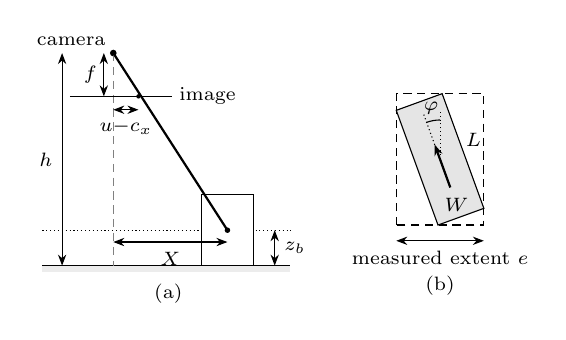
\begin{tikzpicture}[>={Stealth[length=1.4mm]}, font=\scriptsize]
% (a) nadir projection
\begin{scope}
  \fill[gray!15] (-0.9,-0.08) rectangle (2.25,0);
  \draw (-0.9,0) -- (2.25,0);
  \coordinate (C) at (0,2.7);
  \fill (C) circle (1.2pt) node[above left=-1pt] {camera};
  \draw[densely dashed, gray] (C) -- (0,0);
  \draw (-0.55,2.15) -- (0.75,2.15) node[right=-1pt] {image};
  \coordinate (p) at (0.32,2.15);
  \fill (p) circle (0.8pt);
  \draw[densely dotted] (-0.9,0.45) -- (2.25,0.45);
  \draw[fill=white] (1.12,0) rectangle (1.78,0.9);
  \coordinate (Q) at (1.45,0.45);
  \draw[thick] (C) -- (Q);
  \fill (Q) circle (1pt);
  \draw[<->] (-0.65,0) -- node[left] {$h$} (-0.65,2.7);
  \draw[<->] (-0.12,2.7) -- node[left=-1pt] {$f$} (-0.12,2.15);
  \draw[<->] (0,1.98) -- node[below] {$u{-}c_x$} (0.32,1.98);
  \draw[<->] (0,0.3) -- node[below] {$X$} (1.45,0.3);
  \draw[<->] (2.05,0) -- node[right] {$z_b$} (2.05,0.45);
  \node at (0.7,-0.35) {(a)};
\end{scope}
% (b) bounding-box extent of a heading vehicle
\begin{scope}[xshift=4.15cm, yshift=1.35cm]
  \pgfmathsetmacro{\W}{0.62}\pgfmathsetmacro{\L}{1.55}\pgfmathsetmacro{\ph}{20}
  \pgfmathsetmacro{\hx}{(\W*cos(\ph)+\L*sin(\ph))/2}
  \pgfmathsetmacro{\hy}{(\W*sin(\ph)+\L*cos(\ph))/2}
  \draw[densely dashed] (-\hx,-\hy) rectangle (\hx,\hy);
  \begin{scope}[rotate=\ph]
    \draw[fill=gray!20] (-\W/2,-\L/2) rectangle (\W/2,\L/2);
    \draw[->, thick] (0,-0.38) -- (0,0.2);
    \node[right=-1pt] at (\W/2,0.15) {$L$};
    \node at (0,-\L/2+0.16) {$W$};
    \draw[densely dotted] (0,0) -- (0,0.62);
  \end{scope}
  \draw[densely dotted] (0,0) -- (0,0.62);
  \draw (0,0.5) arc[start angle=90, end angle=90+\ph, radius=0.5];
  \node at (100:0.66) {$\varphi$};
  \draw[<->] (-\hx,-\hy-0.2) -- node[below] {measured extent $e$} (\hx,-\hy-0.2);
  \node at (0,-1.6) {(b)};
\end{scope}
\end{tikzpicture}
\caption{(a) Nadir projection: by similar triangles, a pixel offset $u{-}c_x$ maps to a ground offset $X = (h{-}z_b)(u{-}c_x)/f$, so only the ratio of height to focal length matters. (b) A vehicle heading at angle $\varphi$ to the image axis fills an axis-aligned box whose extent $e = W|\cos\varphi| + L|\sin\varphi|$ is never smaller than its width $W$.}
\label{fig:geometry}
\end{figure}

\subsection{Scale Self-Calibration from Vehicle Width}

The scale is estimated from the cars in the scene, whose widths vary only within a narrow range. Only vehicles classified as cars are used, since vans, trucks, and buses differ widely in size. During a short calibration clip, the two lower corners of each tracked box are back-projected with a unit camera height, giving the normalised edge length
\begin{equation}
w_i = \frac{|u_2 - u_1|}{f}.
\end{equation}
When this edge spans the width $W$ of a car whose body sides lie at height $z_b$ above the road, $|u_2-u_1| = fW/(h-z_b)$, so $w_i = W/(h-z_b)$ and the camera height follows as $h = W/w_i + z_b$.

Two effects must be handled. First, an axis-aligned box spans the width of a vehicle only when the vehicle travels perpendicular to the measured edge. For a vehicle of length $L$ whose heading deviates from this direction by an angle $\varphi$, the measured extent is
\begin{equation}
e(\varphi) = W|\cos\varphi| + L|\sin\varphi| \;\geq\; W,
\label{eq:extent}
\end{equation}
as shown in Fig.~\ref{fig:geometry}b. A sample is therefore accepted only when the direction of travel, taken from the track over a few frames, is close to perpendicular to the edge, i.e.\ $|\cos\theta_i| < 1/2$, where $\theta_i$ is the angle between the edge and the travel direction. The heading is trusted only once the car has moved by a set fraction of its own width, so slow or parked vehicles, whose direction is unknown, are excluded.

Second, the remaining errors, namely small heading deviations, padding of the detected box, and larger vehicles misclassified as cars, can only make the measured width larger, never smaller. Because the error is one-sided, the median is biased upwards, and a lower percentile is used instead:
\begin{equation}
\hat{h} = \frac{W}{P_p\left(\{w_i\}\right)} + z_b,
\label{eq:scale}
\end{equation}
where $P_p$ denotes the $p$-th percentile over all accepted samples. The values of $W$, $z_b$, and $p$ are listed in Table~\ref{tab:params}.

\subsection{Drift Compensation}

A hovering UAV drifts and rotates slightly, and even a small image shift is interpreted as vehicle motion, giving parked vehicles a false speed. Each box is therefore mapped back to a fixed reference frame before projection:
\begin{equation}
[\tilde{u},\,\tilde{v},\,1]^{\top} \propto \mathbf{H}_t\,[u,\,v,\,1]^{\top},
\end{equation}
where $\mathbf{H}_t$ is the homography from frame $t$ to the reference frame. Because the road is planar, a homography describes this drift exactly for points on the road. $\mathbf{H}_t$ is estimated with RANSAC from ORB feature matches between the two frames, with vehicle boxes masked out so that moving traffic cannot bias the estimate. It is re-estimated at regular intervals and applied only when the displacement it implies is plausible: below a lower bound the camera is treated as static, since applying the fit would only add matching noise, and above an upper bound the match is treated as a failure.

\subsection{Speed Estimation}

The position of each vehicle is the centre of its drift-corrected box, projected with (\ref{eq:nadir}) at the vehicle centroid height $z = z_b$. For each track, the positions $(X_k, Y_k)$ observed at times $\tau_k$ within the last $T$ seconds are fitted with a constant-velocity model by least squares:
\begin{equation}
v_x = \frac{\sum_k (\tau_k-\bar{\tau})(X_k-\bar{X})}{\sum_k (\tau_k-\bar{\tau})^2},
\end{equation}
and similarly for $v_y$. The speed in km/h is
\begin{equation}
v = 3.6\,\sqrt{v_x^2 + v_y^2}.
\end{equation}
Fitting over a window, rather than differencing two consecutive frames, averages out the frame-to-frame jitter of the bounding boxes. The fit also provides the largest residual $r$ and the standard error of the slope $\sigma_{se}$, which are used by the reliability gate.

\subsection{Reliability Gate}

A speed reading is useful only if it can be distinguished from measurement noise. Bounding-box jitter is modelled as a fixed fraction $k$ of the box size. Since the box size in pixels shrinks in proportion to the distance $D$ from the camera, the resulting position error grows linearly with distance:
\begin{equation}
\sigma_{pos} = \frac{kWD}{h}, \qquad \sigma_v = 3.6\,\frac{2\,\sigma_{pos}}{T},
\label{eq:noise}
\end{equation}
where $\sigma_v$ is the corresponding speed uncertainty over the window $T$. For a nadir camera $D \approx h$ for every vehicle in view, so $\sigma_{pos} \approx kW$: under this model the position noise is uniform across the image and independent of flight altitude. In practice the altitude is still limited by the detector, which must be able to resolve each vehicle.

Each reading is assigned one of four states. A track with too few samples is in \textit{warm-up}. With $\sigma = \max(\sigma_{se}, \sigma_v)$, a reading is \textit{unreliable} if
\begin{equation}
v > v_{max} \;\;\lor\;\; r > r_{max} \;\;\lor\;\;
\left(\sigma > v_{stop} \,\land\, v < 2\sigma\right),
\label{eq:gate}
\end{equation}
that is, if it is physically implausible, if the trajectory is inconsistent with constant velocity, or if it cannot be told apart from a stationary vehicle. Otherwise the vehicle is \textit{stopped} if $v < v_{stop}$ and \textit{moving} if not. An unreliable reading is never replaced by zero, so a parked vehicle and a failed measurement always remain distinguishable.

\begin{table}[htbp]
\centering
\caption{Parameters of the method.}
\label{tab:params}
\begin{tabular}{|c|l|c|}
\hline
\textbf{Symbol} & \textbf{Description} & \textbf{Value} \\
\hline
$W$ & Reference car width & 1.83 m \\
$z_b$ & Vehicle centroid height & 0.75 m \\
$p$ & Width percentile & 25 \\
$T$ & Speed fit window & 0.6 s \\
$v_{stop}$ & Stopped threshold & 3 km/h \\
$v_{max}$ & Plausibility limit & 200 km/h \\
$r_{max}$ & Maximum fit residual & 1.5 m \\
$T_{min}$ & Minimum exceedance duration & 0.7 s \\
\hline
\end{tabular}
\end{table}

\subsection{Overspeed Event Logging}

Vehicles exceeding a speed limit $V_L$ are recorded in a cloud PostgreSQL database. To prevent false records from momentary errors, a vehicle is logged only after its reliable speed has stayed above $V_L$ continuously for at least $T_{min}$ seconds; any reading at or below the limit, or any unreliable reading, restarts this count. The duration is defined in seconds rather than frames, so the rule behaves the same at any frame rate. Each vehicle produces a single record, keyed by its track identifier within the recording session, which stores the detection time, vehicle type, camera location, and the peak speed observed; the record is updated only if the peak rises appreciably. An evidence image, cropped around the vehicle before any annotation is drawn, is stored in cloud object storage and linked to the record. Database writes run in a background thread, so a slow or unavailable connection never stalls video processing.

\subsection{System Implementation}

The system is implemented in Python with OpenCV and Ultralytics. It accepts both recorded videos and live streams, and presents the annotated video, the event log, and summary statistics through a web interface. Timestamps are taken from the media position for recorded video and from the system clock for live streams, so measured speeds do not depend on processing rate.

\subsection{Assumptions and Limitations}

The method assumes a flat road and a camera pointing close to straight down. Oblique views violate the nadir model and require full estimation of the road plane, as in \cite{ref2}. The scale rests on a typical car width, so a vehicle fleet with a different average width scales all speeds by the same proportion. In the current implementation the measured edge is the lower edge of each box, so calibration relies on cars travelling roughly along the vertical image axis. Finally, the jitter coefficient $k$ and the thresholds in Table~\ref{tab:params} are set empirically.

% TODO: Section "Results and Analysis" goes here once experiments with
% ground-truth speeds are done; move "Assumptions and Limitations" to its end
% as a "Limitations" subsection, matching the previous paper.

\section{Conclusion}

This paper presented a vehicle speed estimation method for overhead UAV video that derives its metric scale from the traffic itself. For a downward-facing camera, ground positions depend only on the ratio of camera height to focal length, and this ratio can be recovered from the widths of tracked cars once the one-sided bias of axis-aligned boxes is accounted for. Combined with drift compensation, a window-based speed fit, and a reliability gate that keeps stationary vehicles and measurement failures apart, the method produces speed estimates without flight metadata, camera intrinsics, or ground measurements, and logs speeding vehicles with supporting evidence. Future work will validate the method against ground-truth speeds from a GPS-equipped probe vehicle, extend the model to moderately tilted views, use class-specific size priors for vans and trucks, and deploy the pipeline on board the UAV.

% TODO: add funding details, as in the previous paper.
% \section*{Acknowledgment}
%
% This research is funded by ...

\begin{thebibliography}{00}

\bibitem{ref1}
D. Mouafo and U. Biaou, ``Uncalibrated camera approach for vehicle speed estimation using detection and tracking,'' \textit{Signal, Image and Video Processing}, vol. 18, pp. 8819--8827, 2024, doi: 10.1007/s11760-024-03509-2.

\bibitem{ref2}
M. Dubsk\'a, A. Herout, R. Jur\'anek, and J. Sochor, ``Fully automatic roadside camera calibration for traffic surveillance,'' \textit{IEEE Transactions on Intelligent Transportation Systems}, vol. 16, no. 3, pp. 1162--1171, Jun. 2015, doi: 10.1109/TITS.2014.2352854.

\bibitem{ref3}
D. A. Kamil, Wahyono, A. Harjoko, and K.-H. Jo, ``Vehicle speed estimation using consecutive frame approaches and deep image homography for image rectification on monocular videos,'' \textit{IEEE Access}, vol. 12, pp. 181937--181952, 2024, doi: 10.1109/ACCESS.2024.3508135.

\bibitem{ref4}
K. Sangsuwan and M. Ekpanyapong, ``Video-based vehicle speed estimation using speed measurement metrics,'' \textit{IEEE Access}, vol. 12, pp. 4845--4858, 2024, doi: 10.1109/ACCESS.2024.3350381.

\bibitem{ref5}
I. Lashkov, R. Yuan, and G. Zhang, ``Edge-computing-empowered vehicle tracking and speed estimation against strong image vibrations using surveillance monocular camera,'' \textit{IEEE Transactions on Intelligent Transportation Systems}, vol. 24, no. 11, pp. 13486--13502, Nov. 2023, doi: 10.1109/TITS.2023.3318077.

\bibitem{ref6}
Y. Wang and V. Y. Mariano, ``A multi object tracking framework based on YOLOv8s and Bytetrack algorithm,'' \textit{IEEE Access}, vol. 12, pp. 120711--120719, 2024, doi: 10.1109/ACCESS.2024.3450370.

\bibitem{ref7}
E. Bayraktar, ``Advanced Kalman filter optimization for efficient multi-object tracking in computer vision,'' in \textit{2024 Innovations in Intelligent Systems and Applications Conference (ASYU)}, 2024, pp. 1--6, doi: 10.1109/ASYU62119.2024.10757018.

\end{thebibliography}

\end{document}
